\documentclass[ignorenonframetext,]{beamer}
\setbeamertemplate{caption}[numbered]
\setbeamertemplate{caption label separator}{: }
\setbeamercolor{caption name}{fg=normal text.fg}
\beamertemplatenavigationsymbolsempty
\usepackage{lmodern}
\usepackage{amssymb,amsmath}
\usepackage{ifxetex,ifluatex}
\usepackage{fixltx2e} % provides \textsubscript
\ifnum 0\ifxetex 1\fi\ifluatex 1\fi=0 % if pdftex
  \usepackage[T1]{fontenc}
  \usepackage[utf8]{inputenc}
\else % if luatex or xelatex
  \ifxetex
    \usepackage{mathspec}
  \else
    \usepackage{fontspec}
  \fi
  \defaultfontfeatures{Ligatures=TeX,Scale=MatchLowercase}
\fi
% use upquote if available, for straight quotes in verbatim environments
\IfFileExists{upquote.sty}{\usepackage{upquote}}{}
% use microtype if available
\IfFileExists{microtype.sty}{%
\usepackage{microtype}
\UseMicrotypeSet[protrusion]{basicmath} % disable protrusion for tt fonts
}{}
\newif\ifbibliography
\hypersetup{
            pdftitle={Lecture 7: GLMs: Score equations, Residuals},
            pdfauthor={Nick Reich / Transcribed by Bing Miu and Yukun Li},
            pdfborder={0 0 0},
            breaklinks=true}
\urlstyle{same}  % don't use monospace font for urls
\usepackage{color}
\usepackage{fancyvrb}
\newcommand{\VerbBar}{|}
\newcommand{\VERB}{\Verb[commandchars=\\\{\}]}
\DefineVerbatimEnvironment{Highlighting}{Verbatim}{commandchars=\\\{\}}
% Add ',fontsize=\small' for more characters per line
\usepackage{framed}
\definecolor{shadecolor}{RGB}{248,248,248}
\newenvironment{Shaded}{\begin{snugshade}}{\end{snugshade}}
\newcommand{\KeywordTok}[1]{\textcolor[rgb]{0.13,0.29,0.53}{\textbf{#1}}}
\newcommand{\DataTypeTok}[1]{\textcolor[rgb]{0.13,0.29,0.53}{#1}}
\newcommand{\DecValTok}[1]{\textcolor[rgb]{0.00,0.00,0.81}{#1}}
\newcommand{\BaseNTok}[1]{\textcolor[rgb]{0.00,0.00,0.81}{#1}}
\newcommand{\FloatTok}[1]{\textcolor[rgb]{0.00,0.00,0.81}{#1}}
\newcommand{\ConstantTok}[1]{\textcolor[rgb]{0.00,0.00,0.00}{#1}}
\newcommand{\CharTok}[1]{\textcolor[rgb]{0.31,0.60,0.02}{#1}}
\newcommand{\SpecialCharTok}[1]{\textcolor[rgb]{0.00,0.00,0.00}{#1}}
\newcommand{\StringTok}[1]{\textcolor[rgb]{0.31,0.60,0.02}{#1}}
\newcommand{\VerbatimStringTok}[1]{\textcolor[rgb]{0.31,0.60,0.02}{#1}}
\newcommand{\SpecialStringTok}[1]{\textcolor[rgb]{0.31,0.60,0.02}{#1}}
\newcommand{\ImportTok}[1]{#1}
\newcommand{\CommentTok}[1]{\textcolor[rgb]{0.56,0.35,0.01}{\textit{#1}}}
\newcommand{\DocumentationTok}[1]{\textcolor[rgb]{0.56,0.35,0.01}{\textbf{\textit{#1}}}}
\newcommand{\AnnotationTok}[1]{\textcolor[rgb]{0.56,0.35,0.01}{\textbf{\textit{#1}}}}
\newcommand{\CommentVarTok}[1]{\textcolor[rgb]{0.56,0.35,0.01}{\textbf{\textit{#1}}}}
\newcommand{\OtherTok}[1]{\textcolor[rgb]{0.56,0.35,0.01}{#1}}
\newcommand{\FunctionTok}[1]{\textcolor[rgb]{0.00,0.00,0.00}{#1}}
\newcommand{\VariableTok}[1]{\textcolor[rgb]{0.00,0.00,0.00}{#1}}
\newcommand{\ControlFlowTok}[1]{\textcolor[rgb]{0.13,0.29,0.53}{\textbf{#1}}}
\newcommand{\OperatorTok}[1]{\textcolor[rgb]{0.81,0.36,0.00}{\textbf{#1}}}
\newcommand{\BuiltInTok}[1]{#1}
\newcommand{\ExtensionTok}[1]{#1}
\newcommand{\PreprocessorTok}[1]{\textcolor[rgb]{0.56,0.35,0.01}{\textit{#1}}}
\newcommand{\AttributeTok}[1]{\textcolor[rgb]{0.77,0.63,0.00}{#1}}
\newcommand{\RegionMarkerTok}[1]{#1}
\newcommand{\InformationTok}[1]{\textcolor[rgb]{0.56,0.35,0.01}{\textbf{\textit{#1}}}}
\newcommand{\WarningTok}[1]{\textcolor[rgb]{0.56,0.35,0.01}{\textbf{\textit{#1}}}}
\newcommand{\AlertTok}[1]{\textcolor[rgb]{0.94,0.16,0.16}{#1}}
\newcommand{\ErrorTok}[1]{\textcolor[rgb]{0.64,0.00,0.00}{\textbf{#1}}}
\newcommand{\NormalTok}[1]{#1}
\usepackage{longtable,booktabs}
\usepackage{caption}
% These lines are needed to make table captions work with longtable:
\makeatletter
\def\fnum@table{\tablename~\thetable}
\makeatother
\usepackage{graphicx,grffile}
\makeatletter
\def\maxwidth{\ifdim\Gin@nat@width>\linewidth\linewidth\else\Gin@nat@width\fi}
\def\maxheight{\ifdim\Gin@nat@height>\textheight0.8\textheight\else\Gin@nat@height\fi}
\makeatother
% Scale images if necessary, so that they will not overflow the page
% margins by default, and it is still possible to overwrite the defaults
% using explicit options in \includegraphics[width, height, ...]{}
\setkeys{Gin}{width=\maxwidth,height=\maxheight,keepaspectratio}

% Prevent slide breaks in the middle of a paragraph:
\widowpenalties 1 10000
\raggedbottom

\AtBeginPart{
  \let\insertpartnumber\relax
  \let\partname\relax
  \frame{\partpage}
}
\AtBeginSection{
  \ifbibliography
  \else
    \let\insertsectionnumber\relax
    \let\sectionname\relax
    \frame{\sectionpage}
  \fi
}
\AtBeginSubsection{
  \let\insertsubsectionnumber\relax
  \let\subsectionname\relax
  \frame{\subsectionpage}
}

\setlength{\parindent}{0pt}
\setlength{\parskip}{6pt plus 2pt minus 1pt}
\setlength{\emergencystretch}{3em}  % prevent overfull lines
\providecommand{\tightlist}{%
  \setlength{\itemsep}{0pt}\setlength{\parskip}{0pt}}
\setcounter{secnumdepth}{0}
%       ************************************************
%       **        LaTeX preamble to be used with all 
%	**        statsTeachR labs/handouts.
%
%	Author: Nicholas G Reich
%	Last modified: July 2017
%	************************************************

%\documentclass[table]{beamer}

%	Set theme (a nice plain one)
\usetheme{Malmoe}

%	Use named colors, set main color of theme
%		to match Web site color:
\definecolor{MainColor}{RGB}{10, 74, 109}
\colorlet{MainColorMedium}{MainColor!50}
\colorlet{MainColorLight}{MainColor!20}
\usecolortheme[named=MainColor]{structure} 

%	For tables
%[dvipsnames] [table]
\usepackage{xcolor}

%% calling tabu.sty, assuming a particular directory structure
\usepackage{../../slide-includes/tabu}	% Even fancier than tabulary
\usepackage{multirow}

%	Just for the degree symbol
\usepackage{textcomp}

%	Get rid of footline (page, author, etc. on each slide)
\setbeamertemplate{footline}{}
%	Get rid of navigation buttons
\setbeamertemplate{navigation symbols}{}

%	Make footnotes not ugly
\usepackage{hanging}
\setbeamertemplate{footnote}{\raggedright\hangpara{1em}{1}\makebox[1em][l]{\insertfootnotemark}\footnotesize\insertfootnotetext\par}

%	Text style for code snippets inline in text:
\newcommand{\codeInline}[1]{\texttt{#1}}

%	Text style for emphasis stronger than \emph:
%		(Note, this doesn't toggle the way \emph does.
%			(Note, this can be done, didn't seem worth the trouble.))
\newcommand{\strong}[1]{{\bfseries{#1}}}


%        ******	Define title page	**********************
\setbeamertemplate{title page}{
	{\color{MainColor}
	% There must be a better way than this -vspace at
	%	 the top and bottom of the page to reduce the 
	%	 bottom margin, but I can't find one that works.
	%\vspace{-6em}

% 	% Go to a lot of trouble to get the title in a
% 	%	nice box, since customizing a beamer block
% 	%	does not entirely work here (I don't know why)
	\newlength{\titleBoxWidth}
	\setlength{\titleBoxWidth}{\textwidth}
	\addtolength{\titleBoxWidth}{-2.0em}
	\setlength{\fboxsep}{1.0em}
	\setlength{\fboxrule}{0pt}
	\fcolorbox{MainColor!25}{MainColor!25}{
		\parbox{\titleBoxWidth}{
			\raggedright
			\LARGE\textbf{\inserttitle}
		}	% end parbox
	}	% end fcolorbox

	\vfill
	\small{Author: \insertauthor}
	\vspace{\baselineskip}

	\small{Course: \underline{\href{http://nickreich.github.io/cda}{Categorical Data Analysis}} (BIOSTATS 743)}

%	\small{\Instructor}
%	\vspace{\baselineskip}

%	\small{\emph{This material is part of the \strong{statsTeachR} project}}

	\vfill
	
	\tiny{\emph{Made available under the \underline{\href{http://creativecommons.org/licenses/by-sa/4.0/}{Creative Commons Attribution-ShareAlike 4.0 International License}.}} \hfill \includegraphics[height=1em]{../../slide-includes/by-sa-compact.png}
 }


		\vspace{-15em}

	}	% end color
	\clearpage
}	% end define title page

\input{../../slide-includes/shortcuts}

\hypersetup{colorlinks,linkcolor=,urlcolor=MainColor}

\title{Lecture 7: GLMs: Score equations, Residuals}
\author{Nick Reich / Transcribed by Bing Miu and Yukun Li}
\date{}

\begin{document}
\frame{\titlepage}

\begin{frame}{Likelihood Equations for GLMs}

\begin{itemize}
\item
  The GLM likelihood function is given as follows: \[
  \begin{aligned}
  L(\overset{\rightharpoonup}{\beta})
  &= \sum_i log (f(y_i | \theta_i, \phi))\\
  &= \sum_i \Big\{\frac{y_i\theta_i - b(\theta_i)}{a(\phi)} + C(y_i, \phi) \Big\} \\
  &= \sum_i \frac{y_i\theta_i - b(\theta_i)}{a(\phi)} + \sum_i C(y_i, \phi)
  \end{aligned}
  \]
\item
  \(\phi\) is a dispersion parameter. Not indexed by \(i\), assumed to
  be fixed
\item
  \(\theta_i\) contains \(\beta\), from \(\eta_i\)
\item
  \(C(y_i, \phi)\) is from the random component.
\end{itemize}

\end{frame}

\begin{frame}{Score Equations}

\begin{itemize}
\tightlist
\item
  Taking the derivative of the log likelihood function, set it equal to
  0
  \[ \frac{\partial L(\overset{\rightharpoonup}{\beta}) }{\partial \beta_j} = \sum_i\frac{\partial L_i}{\partial \beta_j} = 0, \forall j\]
\item
  Since
  \(\frac{\partial L_i}{\partial\theta_i} = \frac{(y_i-\mu_i)}{a(\phi)}\),
  \(\mu_i=b^\prime(\theta_i)\),
  \(Var(Y_i)=b^{\prime \prime} (\theta_i)a(\phi)\), and
  \(\eta_i=\sum_j\beta_jx_{ij}\) \[
  \begin{aligned}
  0 &= \sum_i\frac{\partial L_i}{\partial \beta_j} = \sum_{i}\frac{y_i-\mu_i}{a(\phi)} \frac{a(\phi)}{Var(Y_i)} \frac{\partial \mu_i}{\partial\eta_i} x_{ij} \\
  &=\sum_{i}\frac{(y_i - \mu_i)x_{ij}}{Var(Y_i)}\frac{\partial \mu_i}{\partial \eta_i}
  \end{aligned}
  \]
\item
  \(V(\theta)= b^{\prime \prime} (\theta)\),
  \(b^{\prime \prime} (\theta)\) is the variance function of the GLM.
\item
  \(\mu_i=E[Y_i|x_i] = g^{-1}(X_i\beta)\). These functions are typically
  non-linear with respect to \(\beta\)'s, thus require iterative
  computation solutions.
\end{itemize}

\end{frame}

\begin{frame}{Example: Score Equation from Binomial GLM (Ch5.5.1)}

Y\textasciitilde{} \(Binomial (n_i, \pi_i)\)

\begin{itemize}
\tightlist
\item
  The joint probability mass function: \[
  \prod_{i=1}^N \pi(x_i)^{y_i}[1-\pi(x_i)]^{n_i-y_i}
  \]
\item
  The log likelihood:
  \[L(\beta) = \sum_j\Big(\sum_iy_ix_{ij}\Big)\beta_j-\sum_in_ilog\Big[1+ exp \Big(\sum_j\beta_jx_{ij}\Big)\Big]
  \]
\item
  The score equation:
  \[\frac{\partial L(\overset{\rightharpoonup}{\beta})}{\partial \beta_j} = \sum_i (y_i - n_i\hat{\pi_i})x_{ij} \qquad \text{note that  }\hat\pi_i = \frac{e^{X_i\beta}}{1 + e^{X_i\beta}}\].
\end{itemize}

\end{frame}

\begin{frame}{Asymptotic Covariance of \(\hat\beta\):}

\begin{itemize}
\item
  The likelihood function determines the asymptotic covariance of the ML
  estimate for \(\hat\beta\).
\item
  Given the information matrix, \(\mathcal{I}\) with \(hj\) elements:
  \[ \mathcal{I} = E\Big[\frac{-\partial^2 L(\overset{\rightharpoonup}{\beta})}{\partial \beta_h \beta_j} \Big] = \sum_{i = 1}^N \frac{x_{ih}x_{ij}}{Var(Y_i)} \Big(\frac{\partial \mu_i}{\partial \eta_i} \Big)^2\]
  where \(w_i\) denotes
  \[w_i = \frac{1}{Var(Y_i)} \Big(\frac{\partial \mu_i}{\partial \eta_i} \Big)^2\]
\end{itemize}

\end{frame}

\begin{frame}{Asymptotic Covariance Matrix of \(\hat\beta\):}

\begin{itemize}
\tightlist
\item
  The information matrix, \(\mathcal{I}\) is equivalent to:
  \(\mathcal{I} = \sum_{i=1}^N x_{ih}x_{ij}w_i = X^TWX\)
\item
  W is a diagonal matrix with \(w_i\) as the diagonal element. In
  practice, W is evulated at \(\hat{\beta}^{MLE}\) and depdent on the
  link function
\item
  The square root of the main diagonal elements of \((X^TWX)^{-1}\) are
  estimated standard errors of \(\hat{\beta}\)
\end{itemize}

\end{frame}

\begin{frame}{Analogous to SLR}

\begin{longtable}[]{@{}lll@{}}
\toprule
\begin{minipage}[b]{0.16\columnwidth}\raggedright\strut
~\strut
\end{minipage} & \begin{minipage}[b]{0.16\columnwidth}\raggedright\strut
SLR\strut
\end{minipage} & \begin{minipage}[b]{0.41\columnwidth}\raggedright\strut
GLM\strut
\end{minipage}\tabularnewline
\midrule
\endhead
\begin{minipage}[t]{0.16\columnwidth}\raggedright\strut
\(Var(\hat{\beta_i})\)\strut
\end{minipage} & \begin{minipage}[t]{0.16\columnwidth}\raggedright\strut
\(\frac{\hat{\sigma}^2}{\sum_{i=1}^N(x_i-\bar{x})^2}\)\strut
\end{minipage} & \begin{minipage}[t]{0.41\columnwidth}\raggedright\strut
the \(i^{th}\) main diagnal element of \((X^TWX)^{-1}\)\strut
\end{minipage}\tabularnewline
\begin{minipage}[t]{0.16\columnwidth}\raggedright\strut
\(Cov(\hat{\beta_i})\)\strut
\end{minipage} & \begin{minipage}[t]{0.16\columnwidth}\raggedright\strut
\(\hat{\sigma}^2(X^TX)^{-1}\)\strut
\end{minipage} & \begin{minipage}[t]{0.41\columnwidth}\raggedright\strut
\((X^TWX)^{-1}\)\strut
\end{minipage}\tabularnewline
\bottomrule
\end{longtable}

\end{frame}

\begin{frame}{Residual and Diagnostics}

\begin{itemize}
\tightlist
\item
  Deviance Tests

  \begin{itemize}
  \tightlist
  \item
    Measure of goodness of fit in GLM based on likelihood
  \item
    Most useful as a comparison between models (used as a screening
    method to identify important covariates)
  \item
    Use the saturated model as a baseline for comparison with other
    model fits
  \item
    For Poisson or binomial GLM: \(D = -2[L(\hat\mu|y)-L(y|y)]\).
  \end{itemize}
\item
  Example of Deviance
\end{itemize}

\begin{longtable}[]{@{}ll@{}}
\toprule
\begin{minipage}[b]{0.14\columnwidth}\raggedright\strut
Model\strut
\end{minipage} & \begin{minipage}[b]{0.47\columnwidth}\raggedright\strut
D(\((y, \hat\mu)\) )\strut
\end{minipage}\tabularnewline
\midrule
\endhead
\begin{minipage}[t]{0.14\columnwidth}\raggedright\strut
Gaussian\strut
\end{minipage} & \begin{minipage}[t]{0.47\columnwidth}\raggedright\strut
\(\sum(Y_i-\hat\mu_i)^2\)\strut
\end{minipage}\tabularnewline
\begin{minipage}[t]{0.14\columnwidth}\raggedright\strut
Poisson\strut
\end{minipage} & \begin{minipage}[t]{0.47\columnwidth}\raggedright\strut
\(2\sum(y_i\text{ln}(\frac{y_i}{\hat\mu_i})-(y_i-\hat\mu_i))\)\strut
\end{minipage}\tabularnewline
\begin{minipage}[t]{0.14\columnwidth}\raggedright\strut
Bionomial\strut
\end{minipage} & \begin{minipage}[t]{0.47\columnwidth}\raggedright\strut
\(2\sum(y_iln(\frac{y_i}{\hat\mu_i})+(n_i-y_i) ln(\frac{n_i-y_i}{n_i-\hat\mu_i}))\)\strut
\end{minipage}\tabularnewline
\bottomrule
\end{longtable}

\end{frame}

\begin{frame}{Deviance tests for nested models}

\begin{itemize}
\item
  Consider two models, \(M_0\) with fitted values \(\hat\mu_0\) and
  \(M_1\) with fitted values \(\hat\mu_1\):
\item
  \(M_0\) is nested within \(M_1\) \[
  \begin{aligned}
  \eta_1^{\mu_1} &= \beta_0+\beta_1X_{11}+\beta_2X_{12} \\
  \eta_0^{\mu_0} &= \beta_0+\beta_1X_{11}
  \end{aligned}
  \]
\item
  Simpler models have smaller log likelihood and larger deviance:
  \(L(\hat\mu_0|y) \le L(\hat\mu_1|y)\) and
  \(D(y|\hat\mu_1) \le D(y|\hat\mu_0)\).
\item
  The likelihood-ratio statistic comparing the two models is the
  difference between the deviances.\\
  \[\begin{aligned}
  -2[L(\hat\mu_0|y)&-L(\hat\mu_1|y)]\\
  &=-2[L(\hat\mu_0|y)-L(y|y)]- \{-2[L(\hat\mu_1|y)-L(y|y)]\}\\
  &=D(y|\hat\mu_0) - D(y|\hat\mu_1)
  \end{aligned}\]
\end{itemize}

\end{frame}

\begin{frame}{Hypothesis test with differences in Deviance}

\begin{itemize}
\tightlist
\item
  \(H_0: \beta_{i1}=...=\beta_{ij} =0\), fit a full and reduced model
\item
  Hypothesis test with difference in deviance as test statistics. df is
  the number of parameter different between \(\mu_1\) and \(\mu_0\) \[
  D(y|\hat\mu_0)-D(y|\hat\mu_1) \sim\chi^2_{df}
  \]
\item
  Reject \(H_0\) if the the chi-square calculated value is larger than
  \(\chi^2_{df, 1-\alpha}\), where df is the number of parameters
  difference between \(\mu_0\) and \(\mu_1\).
\end{itemize}

\end{frame}

\begin{frame}{Residual Examinations}

\begin{itemize}
\item
  Pearson residuals :\\
  \(e_{i}^p=\frac{y-\hat\mu_{i}}{\sqrt{V(\hat\mu_{i})}}\), where
  \(\mu_i=g^{-1}(\eta_i)=g^{-1}(X_i\beta)\)
\item
  Deviance residuals :\\
  \(e_{i}^d= sign(y_i-\hat\mu_i)\sqrt{d_i}\), where \(d_i\) is the
  deviance contribution of \(i_{th}\) obs. and
  \(sign(x)=\begin{cases}1 & x>0\\-1 & x\le0\end{cases}\)
\item
  Standardized residuals:\\
  \(r_{i}= \frac{e_i}{\sqrt{(1- \widehat{h_i}})}\), where
  \(e_i= \frac{y-\hat\mu_i}{\sqrt{V(\hat\mu_{i})}}\), \(\widehat{h_1}\)
  is the measure of leverage, and \(r_i \cong N(0,1)\)
\end{itemize}

\end{frame}

\begin{frame}{Residual Plot}

Problem: Residual plot is hard to interpret for logistic regression

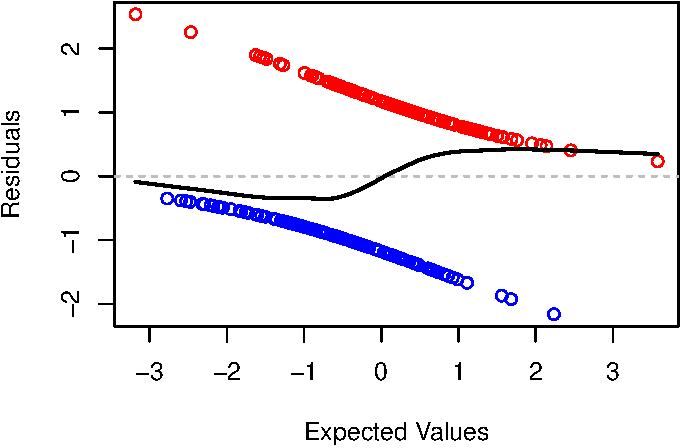
\includegraphics{lec7_files/figure-beamer/unnamed-chunk-1-1.pdf}

\end{frame}

\begin{frame}{Binned Residual Plot}

\begin{itemize}
\tightlist
\item
  Group observations into ordered groups (by \(x_j, \hat{y}\) or
  \(x_{ij}\)), with equal number of observations per group.\\
\item
  Compute group-wise average for raw residuals\\
\item
  Plot the average residuals vs predicted value. Each dot represent a
  group.
\end{itemize}

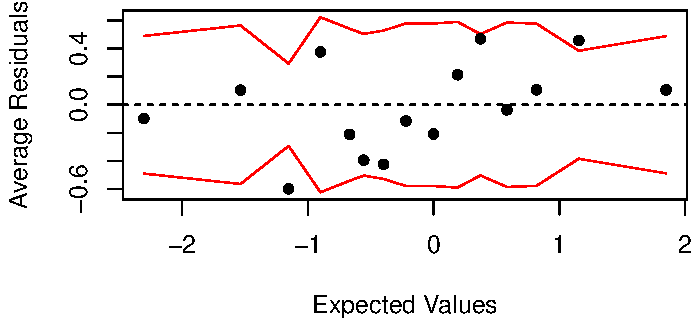
\includegraphics{lec7_files/figure-beamer/unnamed-chunk-2-1.pdf}

\end{frame}

\begin{frame}[fragile]{Binned Residual Plot (Part 2)}

\begin{itemize}
\tightlist
\item
  Red lines indicate \(\pm\) 2 standard-error bounds, within which one
  would expect about 95\% of the binned residuals to fall.
\item
  R function avaiable.
\end{itemize}

\begin{Shaded}
\begin{Highlighting}[]
\KeywordTok{linrary}\NormalTok{(arm)}
\KeywordTok{binnedplot}\NormalTok{(x ,y, nclass...)}
\CommentTok{# x <- Expected values.  # y <- Residuals values.}
\CommentTok{# nclass <- Number of bins.     }
\end{Highlighting}
\end{Shaded}

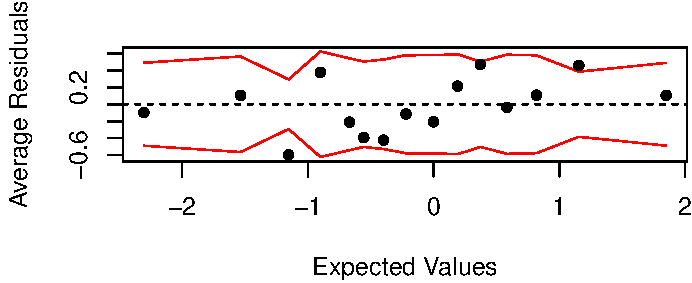
\includegraphics{lec7_files/figure-beamer/unnamed-chunk-4-1.pdf}

\end{frame}

\begin{frame}{Binned Residual Plot (Part 3)}

\begin{itemize}
\tightlist
\item
  In practice may need to fiddle with the number of observations per
  group. Default will take the value of nclass according to the n such
  that:\\
  -- if n \(\ge\) 100, \(nclass=floor(sqrt(length(x)))\);\\
  -- if \(10<n<100\), \(nclass=10\);\\
  -- if \(n<10\), \(nclass=floor(n/2)\).
\end{itemize}

\end{frame}

\begin{frame}{Ex: Binned Residual Plot with different bin sizes}

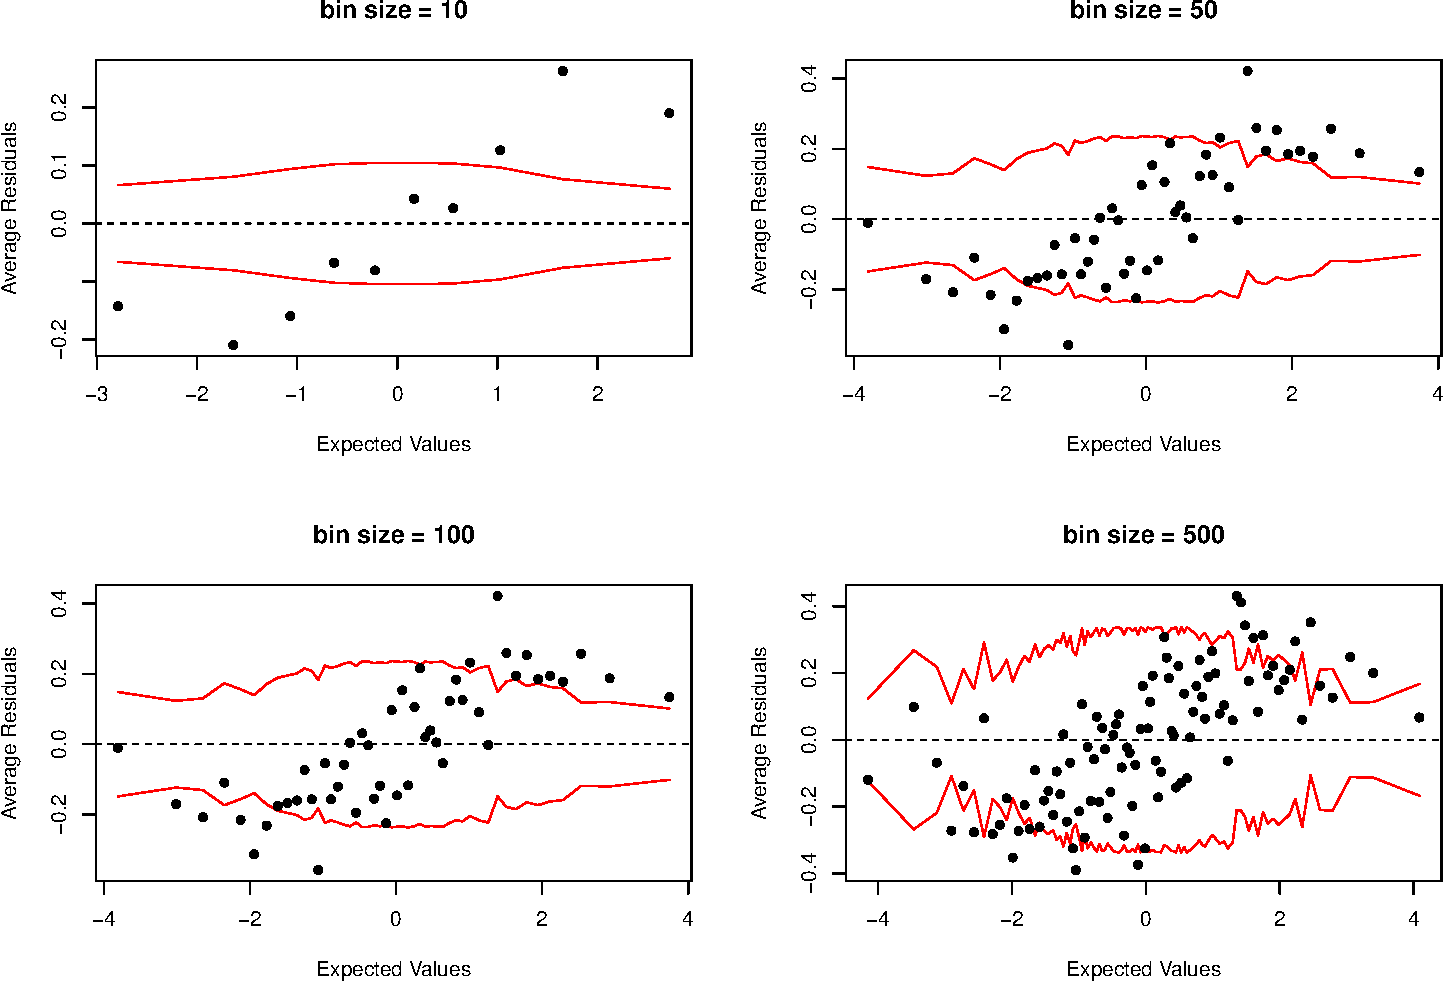
\includegraphics{lec7_files/figure-beamer/unnamed-chunk-5-1.pdf}

\end{frame}

\end{document}
